\section{Messergebnisse und Auswertung}

\subsection{Teil I: Pockels-Effekt}

\subsubsection{Sägezahnmethode}

\begin{figure}[H]
\begin{center}
  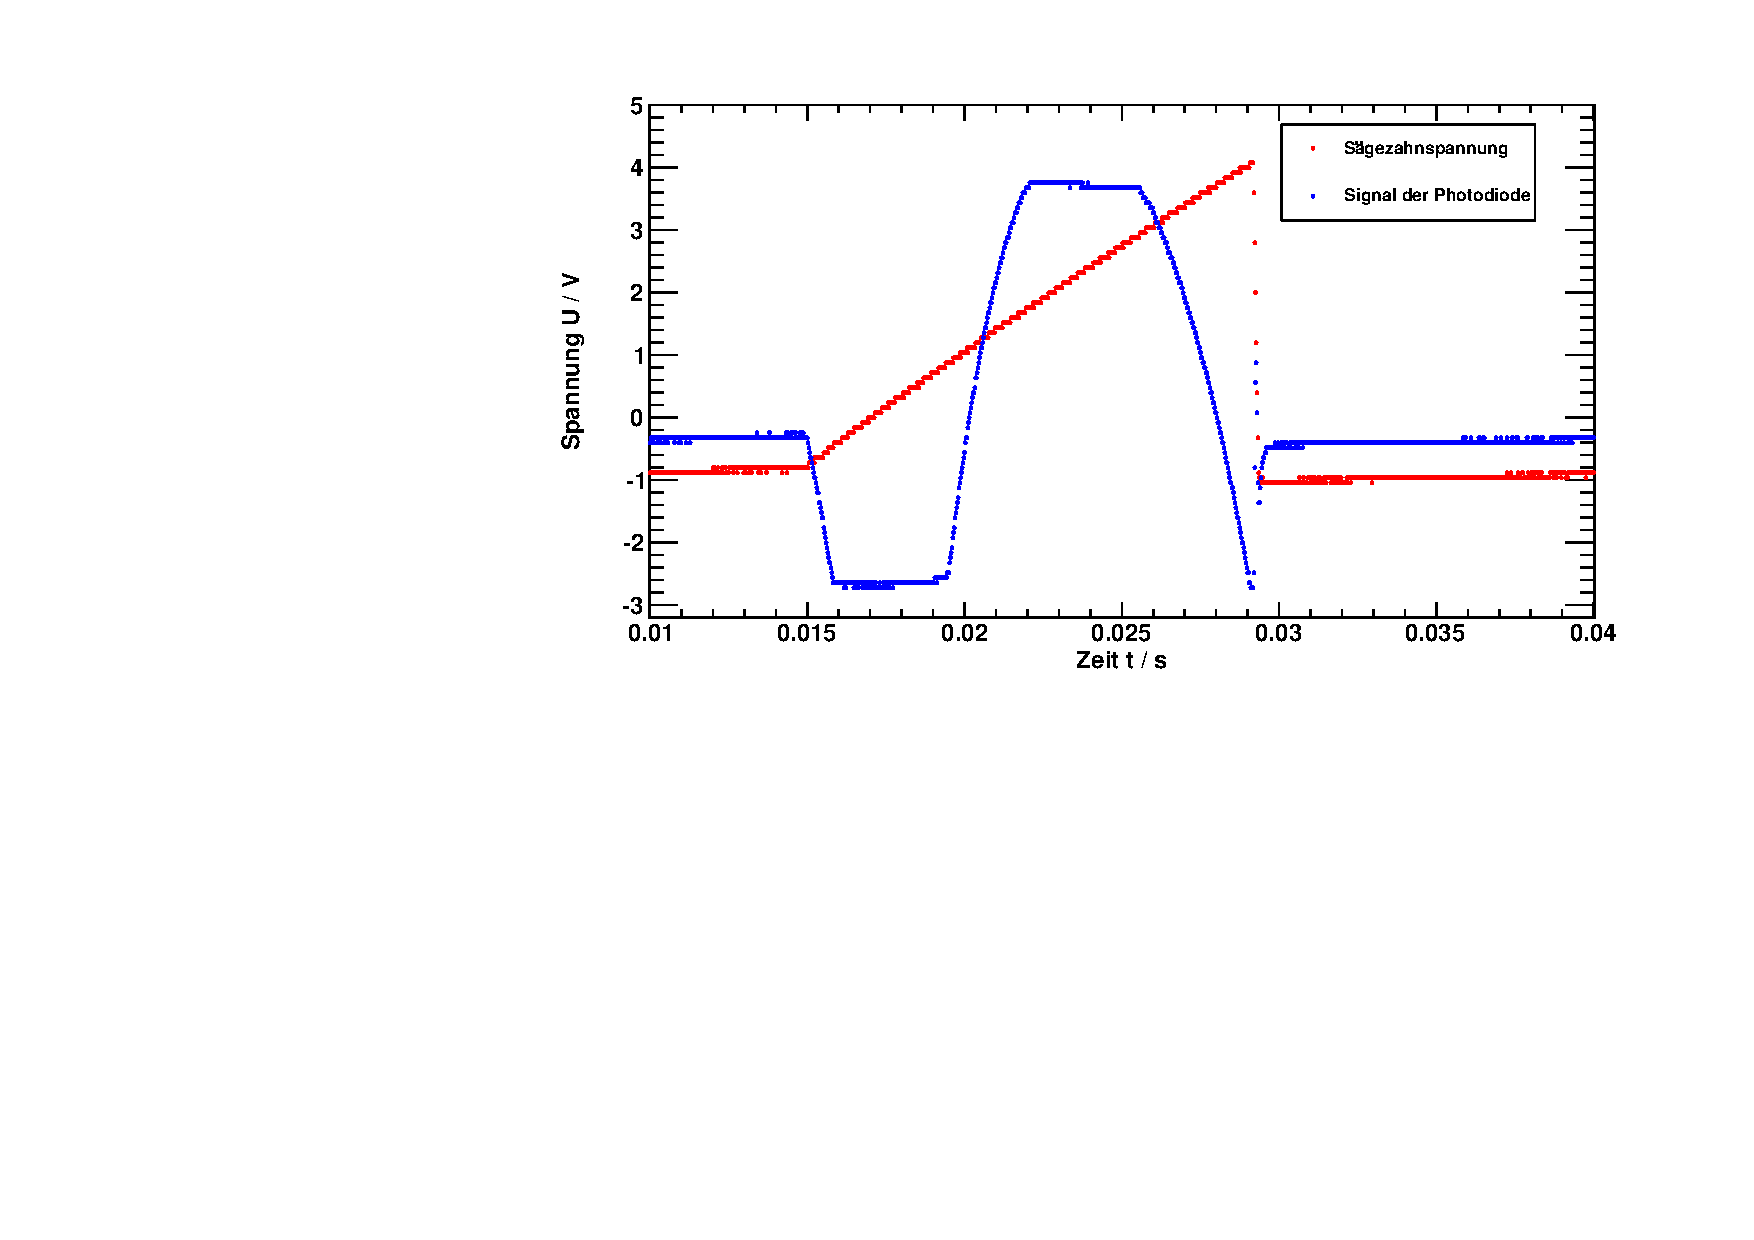
\includegraphics[width=15cm]{../img/pock_saege_winkel0.pdf}
  \caption{Deformiertes Photodiodensignal (blau) bei Einstellung der Achse des Analysators in
  Richtung höchster Transmission der Pockelszelle.}
  \label{img:pock_saege_winkel0}
\end{center}
\end{figure}

\autoref{img:pock_saege_winkel0} zeigt das Photodiodensignal, wenn der Analysator so eingestellt wird,
wie in der Versuchsanleitung beschrieben, so dass die Amplitude des Photodiodensignals maximiert wird.
Diese Einstellung ist zum Ablesen von Maximum und Minimum des Signals nicht geeignet.
\autoref{img:pock_saege_winkel1}, \autoref{img:pock_saege_winkel2} und \autoref{img:pock_saege_winkel3}
zeigen Messungen mit niedrigerer Amplitude, die für die Auswertung verwendet wurden.
In \autoref{tab:minmax} sind die Positionen von Maximum und Minimum für die drei Messungen aufgeführt.
Diese Positionen wurden durch Fits von Parabeln (mit den Fitparametern $a$, $b$ und $s$) an die Messdaten gewonnen:
\begin{equation}
  y = a \cdot (x-s)^2+b
\end{equation}
$s$ ist die Position des Minimums auf der x-Achse.\\
Die Steigung der Sägezahnfunktion wird mit einem Steigungsdreieck abgeschätzt:
Mit den Werten am Einsatzpunkt und am höchsten Punkt der Spannung erhält man folgende Steigung:
\begin{equation}
  m_s = \frac{U_2-U_1}{t_2-t_1} = 50 \,\frac{\text{V}}{\text{s}}
\end{equation}

\begin{figure}[H]
\begin{center}
  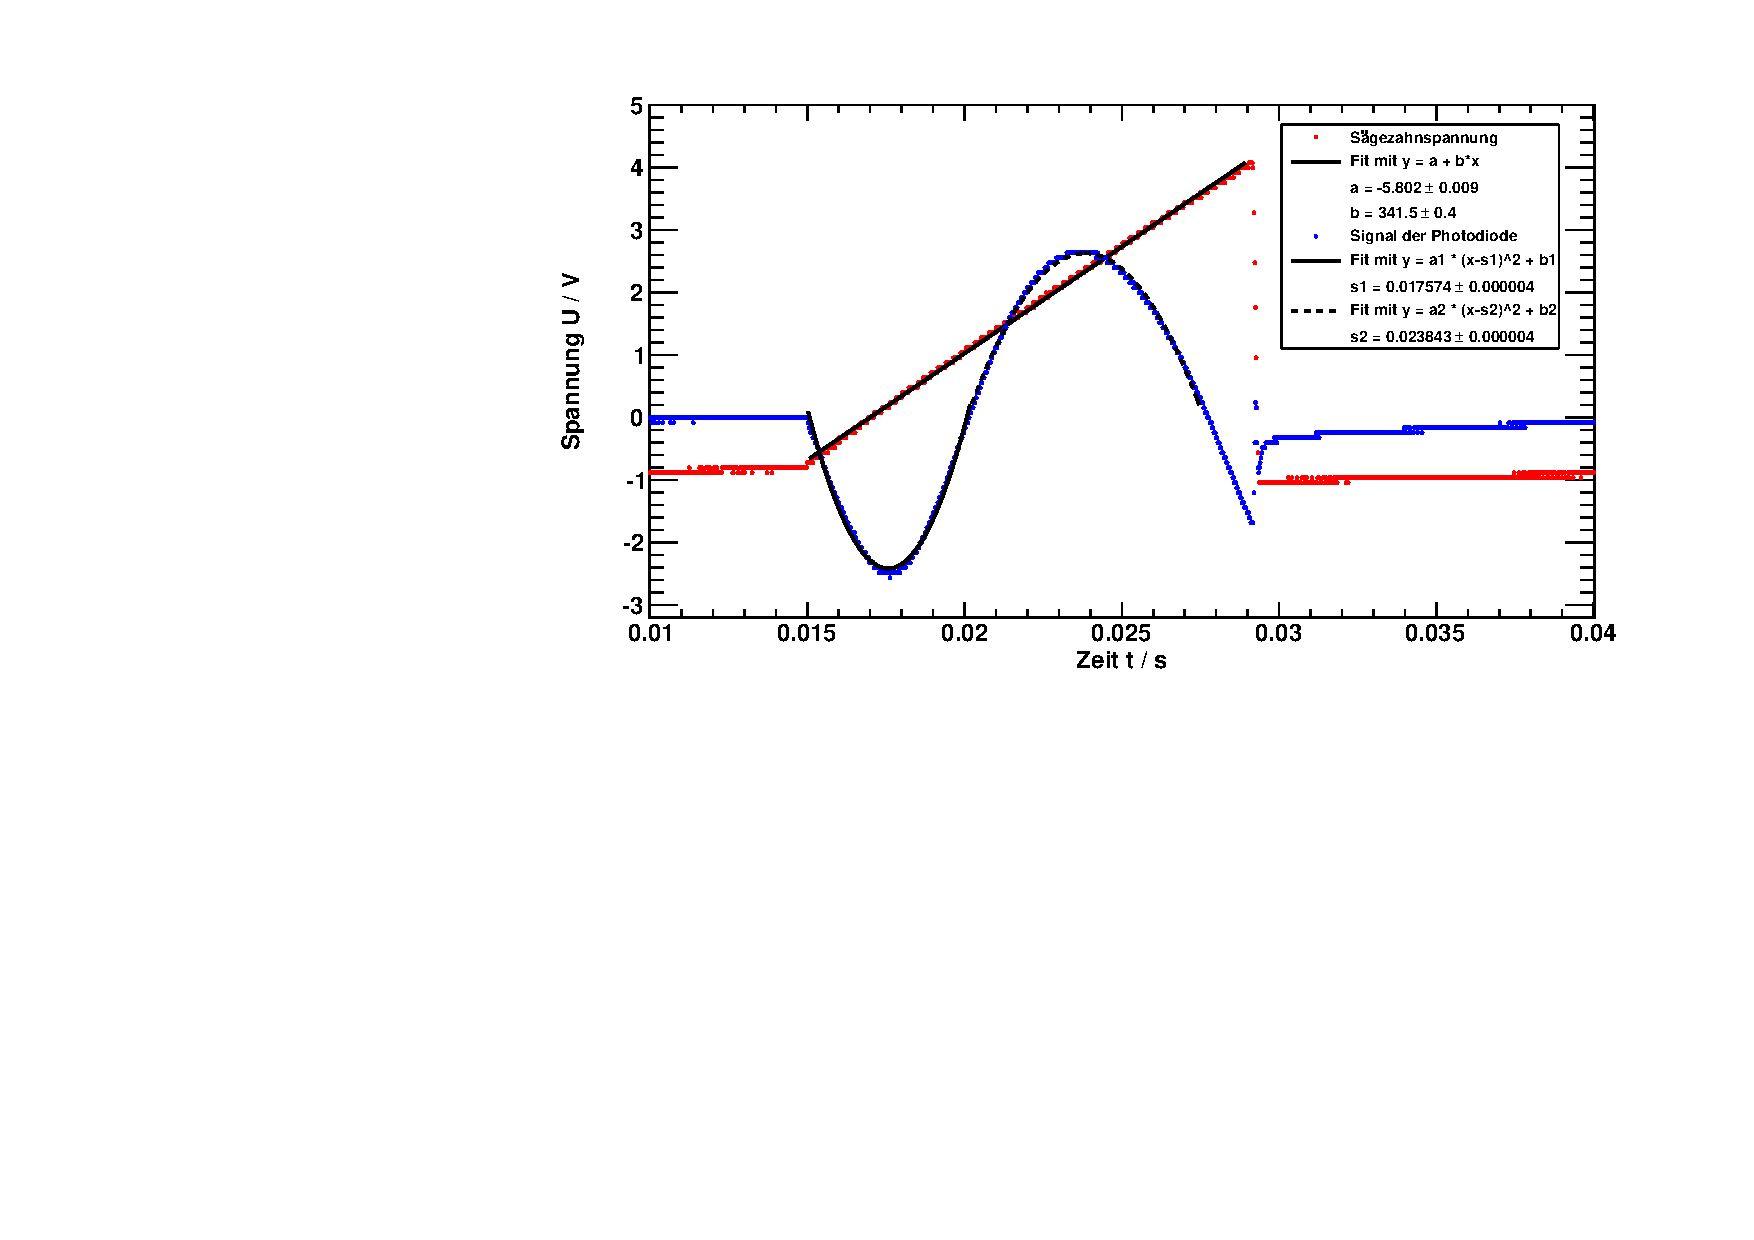
\includegraphics[width=15cm]{../img/pock_saege_winkel1.pdf}
  \caption{capt.}
  \label{img:pock_saege_winkel1}
\end{center}
\end{figure}

\begin{figure}[H]
\begin{center}
  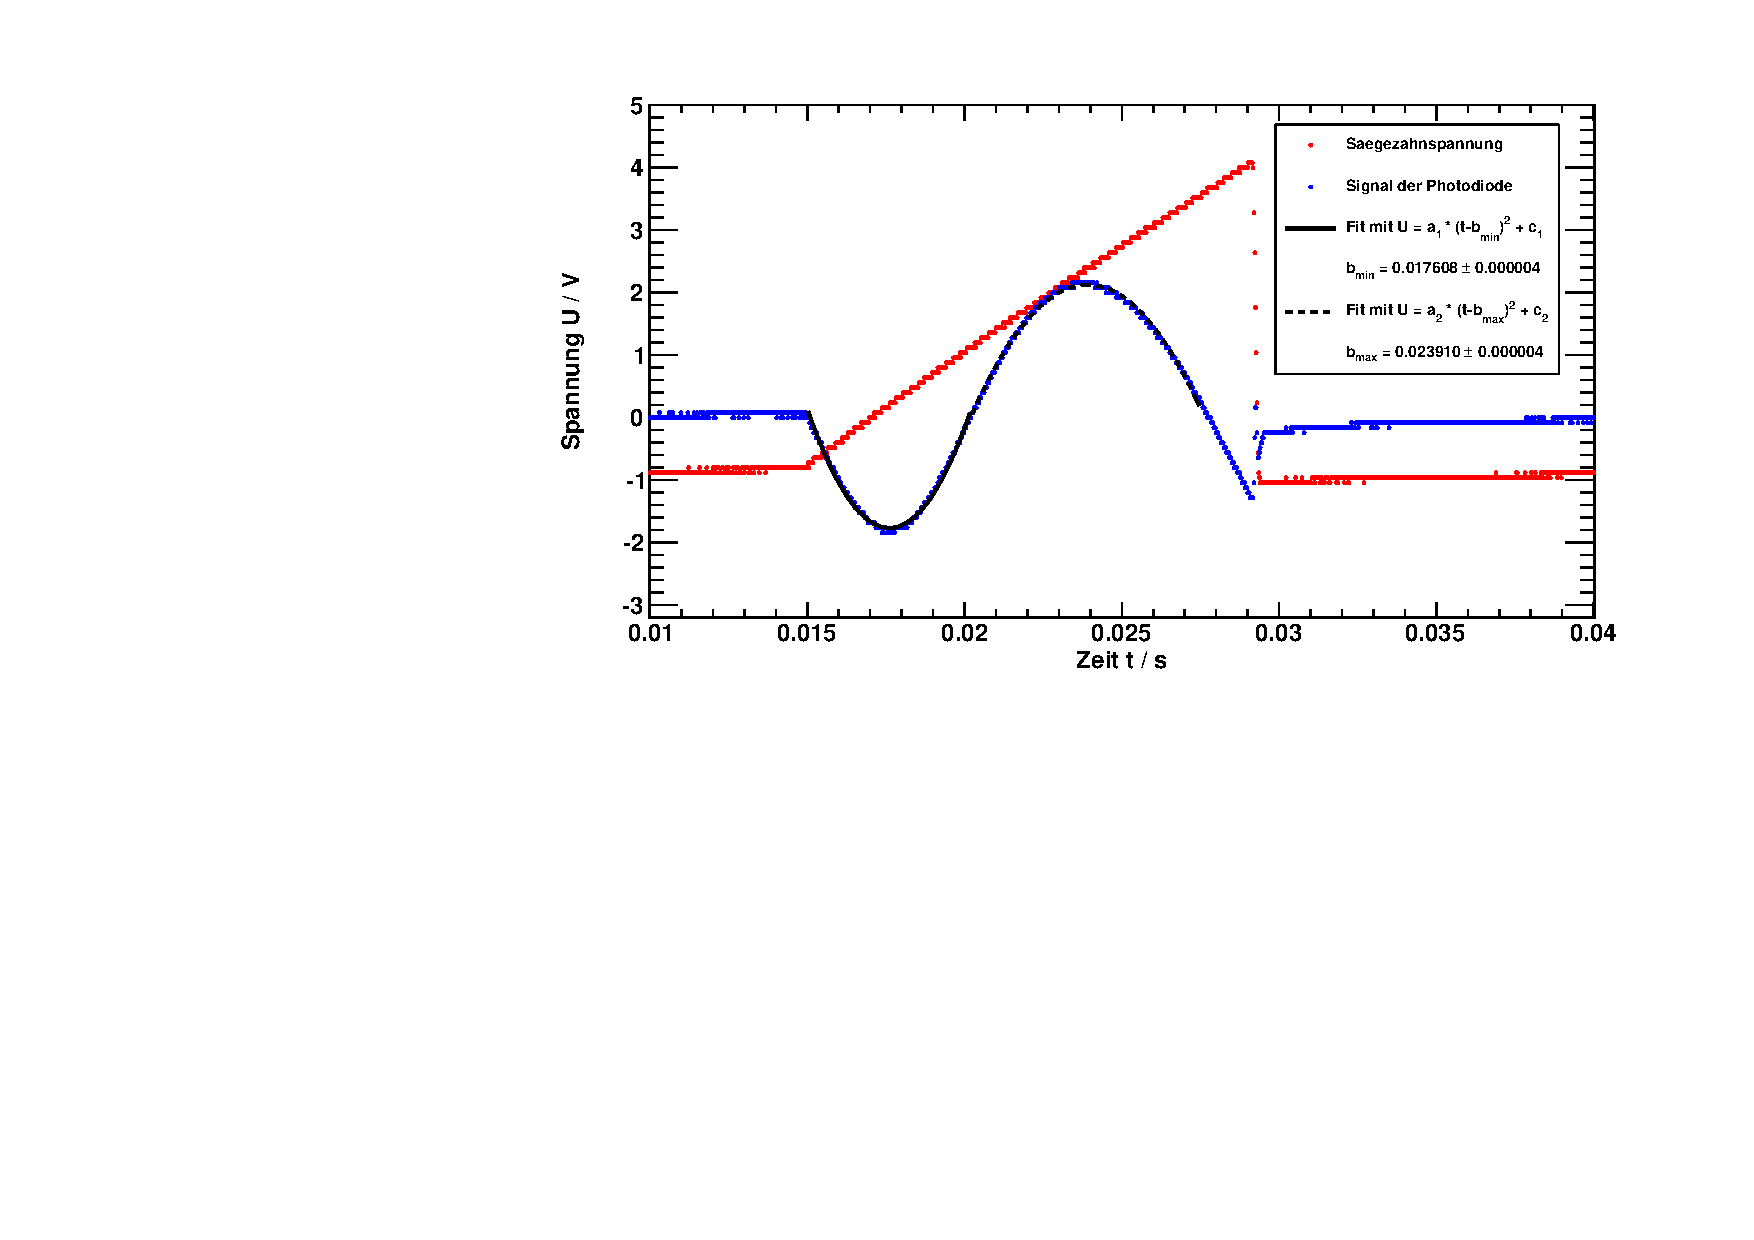
\includegraphics[width=15cm]{../img/pock_saege_winkel2.pdf}
  \caption{capt.}
  \label{img:pock_saege_winkel2}
\end{center}
\end{figure}

\begin{figure}[H]
\begin{center}
  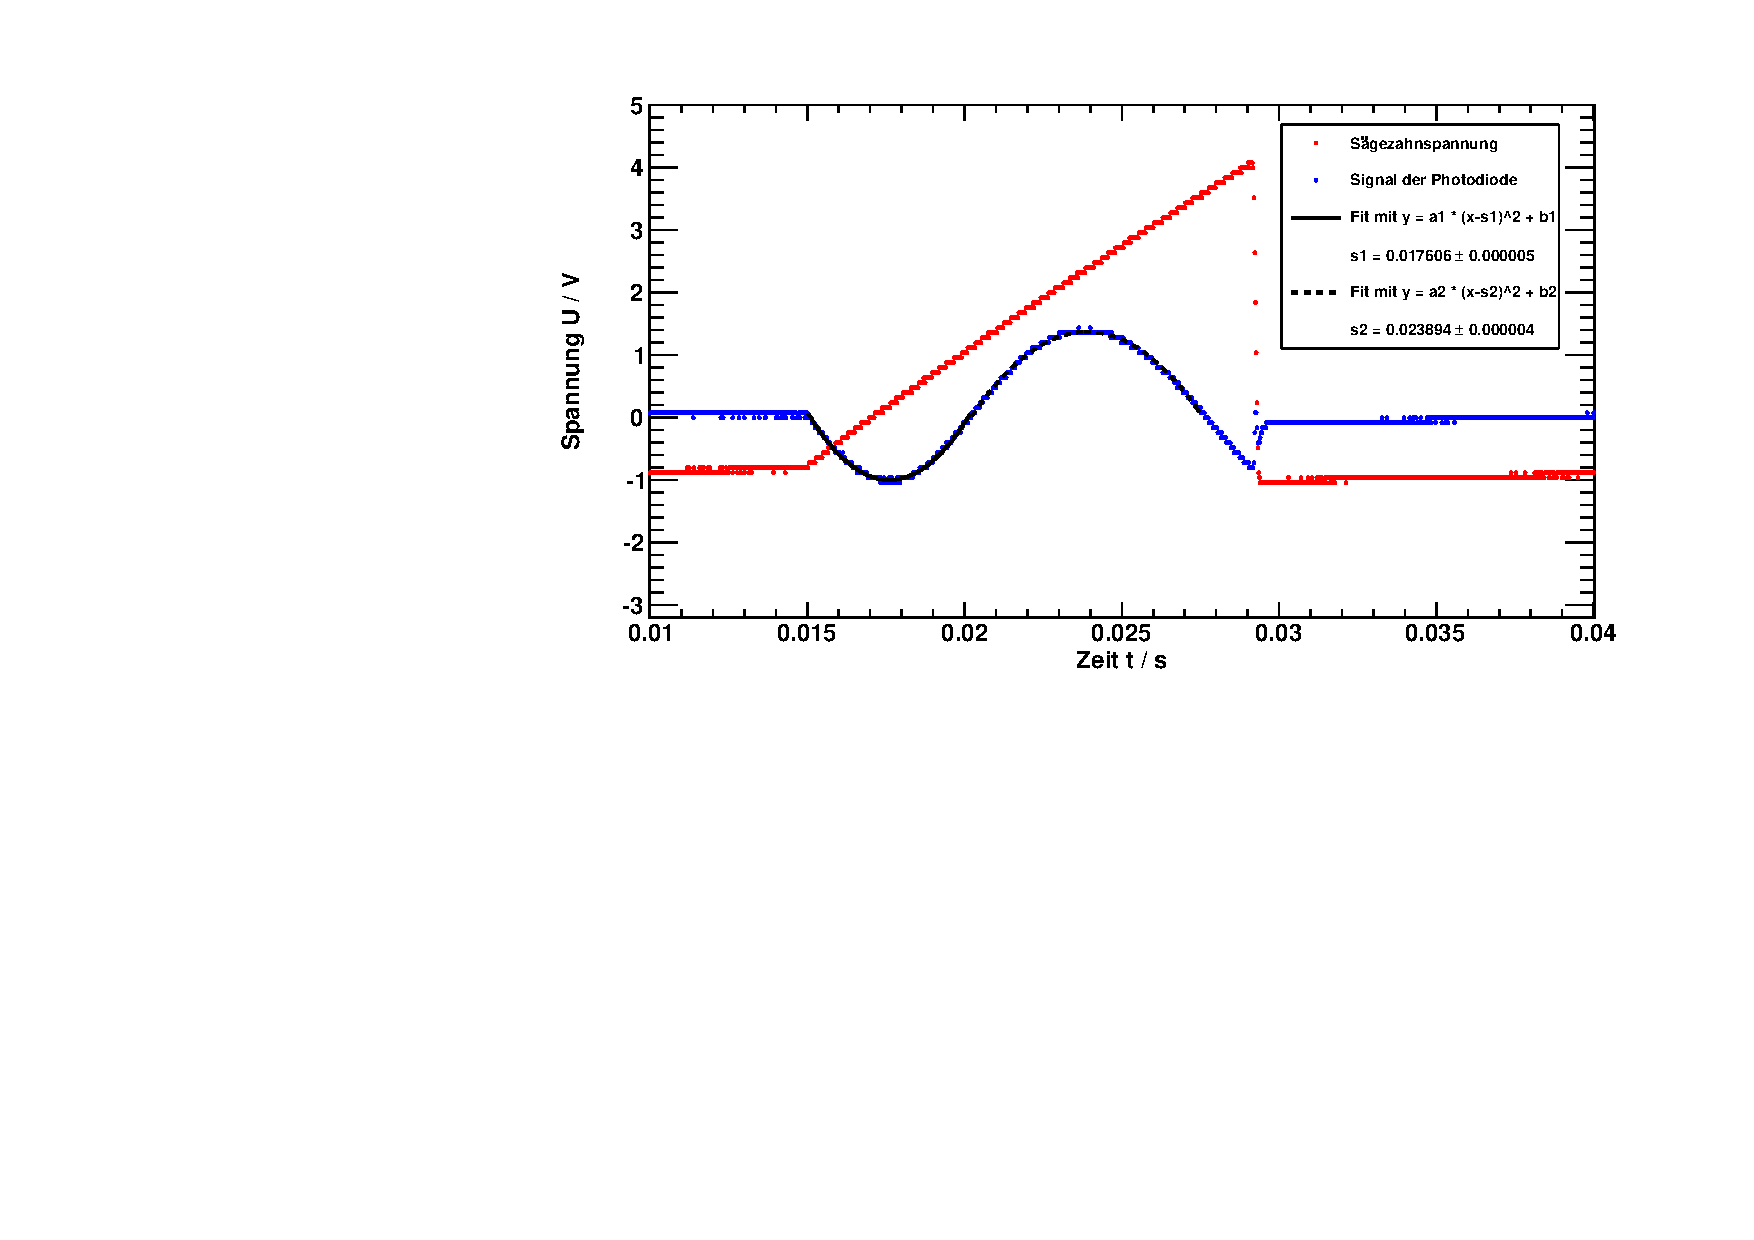
\includegraphics[width=15cm]{../img/pock_saege_winkel3.pdf}
  \caption{capt.}
  \label{img:pock_saege_winkel3}
\end{center}
\end{figure}

\subsubsection{Modulierte Gleichspannung}

\subsection{Teil II: Faraday-Effekt}